\documentclass[a4j, titlepage]{jarticle}

% \usepackage{multirow}
\usepackage[table,xcdraw]{xcolor}
\usepackage[dvipdfmx]{graphicx}
\usepackage{caption}
\usepackage{subcaption}
\usepackage{listings}
\usepackage{fancybox}
\usepackage{ascmac}
\usepackage{amsmath}
\usepackage{longtable}
\usepackage{subfig}

\definecolor{codegreen}{rgb}{0,0.6,0}
\definecolor{codegray}{rgb}{0.5,0.5,0.5}
\definecolor{codepurple}{rgb}{0.58,0,0.82}
\definecolor{backcolour}{rgb}{0.95,0.95,0.92}

% Define a custom style
\lstdefinestyle{mystyle}{
    backgroundcolor=\color{backcolour},   
    commentstyle=\color{codegreen},
    keywordstyle=\color{magenta},
    numberstyle=\tiny\color{codegray},
    stringstyle=\color{codepurple},
    basicstyle=\ttfamily\footnotesize,
    breakatwhitespace=false,         
    breaklines=true,                 
    captionpos=b,                    
    keepspaces=true,                 
    % numbers=left,                    
    numbersep=5pt,                  
    showspaces=false,                
    showstringspaces=false,
    showtabs=false,                  
    tabsize=2,
    frame=single
}

\lstset{style=mystyle}

\begin{document}
  \begin{center}
  \huge 情報工学実験II\par
  \vspace{15mm}
  \huge テーマ03 \par
  \huge グラフ・ネットワークプログラム \par
  \vspace{15mm}
  % \LARGE タイトル \par
  \vspace{20mm}
  \vspace{100mm}
  \Large 令和5年07月06日 \par
  \vspace{15mm}
  \Large イマム カイリ ルビス \par
  \vspace{10mm}
  \Large 学籍番号:214071\par
  \vspace{10mm}
\end{center}
\clearpage

\tableofcontents
\clearpage

\section{概要}
    \subsection{グラフ理論とは}
    数学においてグラフ理論とは,グラフを研究する学問であり,グラフはオブジェクト間の対関係をモデル化するために用いられる数学的構造である.グラフを構成するためには,点(節点またはノードとも呼ばれる)と辺(枝またはエッジとも呼ばれる)が必要である\cite{bib:wikigraph}. 
    % In mathematics, graph theory is the study of graphs, which are mathematical structures used to model pairwise relations between objects. A graph in this context is made up of vertices (also called nodes or points) which are connected by edges (also called links or lines). \ref{bib:wikigraph}
    グラフ理論には,辺が方向を持っているかどうかによって分れている
    \begin{description}
        \item[有向グラフ]:辺の方向が決まっている一方向性のグラフである.
        \item[無向グラフ]:辺が特定の方向を持たず,双方向性を持つグラフである.
    \end{description}
    本実験では,使用したグラフはすべて無向グラフである.更に,

    \subsection{スタックとは} 
    スタックは,データを一時的にた蓄えるためのデータ構造の一つ.データの出し入れは\textbf{後入れ先出し}(\textit{LIFO / Last In First Out})で行われる.すなわち,最後に入れられたデータが最初に取り出される\cite{bib:boyoh}.

    なお,スタックにデータを入れる操作を\textbf{プッシュ}(\textit{push})と呼び,スタックからデータを取り出す操作を\textbf{ポップ}(\textit{pop})と呼びます\cite{bib:boyoh}.% ini jadikan ga ada sitasi aja kali

    しかし本実験では,実際のスタック機能を模倣するため,ノード数分の大きさを持つ配列を使ってスタックデータ構造を作った.

    \subsection{キューとは}
    キューは,データを一時的に蓄えるための基本的なデータ構造の一つである.最初に入れられたデータが最初に取り出されるという\textbf{先入れ先出し}(\textit{FIFO / First In First Out})の機構である.\cite{bib:boyoh}
    
    なお,キューにデータを追加する操作を\textbf{エンキュー}(\textit{enqueue})と呼び,データを取り出す操作を\textbf{デキュー}(\textit{dequeue})と呼ぶ.また,データが取り出される側を\textbf{先頭}(\textit{front})と呼び,データが押し込まれる側を\textbf{末尾}(\textit{rear})と呼ぶ\cite{bib:boyoh}.

    しかし本実験では,実際のキュー機能を模倣するため,ノード数分の大きさを持つ配列を使ってスタックデータ構造を作った.
    \clearpage
        \subsubsection{リングバッファによるキュー}
        リングバッファとは,配列の末尾が先頭につながっているとみなすデータ構造である\cite{bib:boyoh}.エンキューとデキューを行うと\textit{front}と\textit{rear}の値は変化する.
        \begin{figure}[htb]
            \begin{center}
              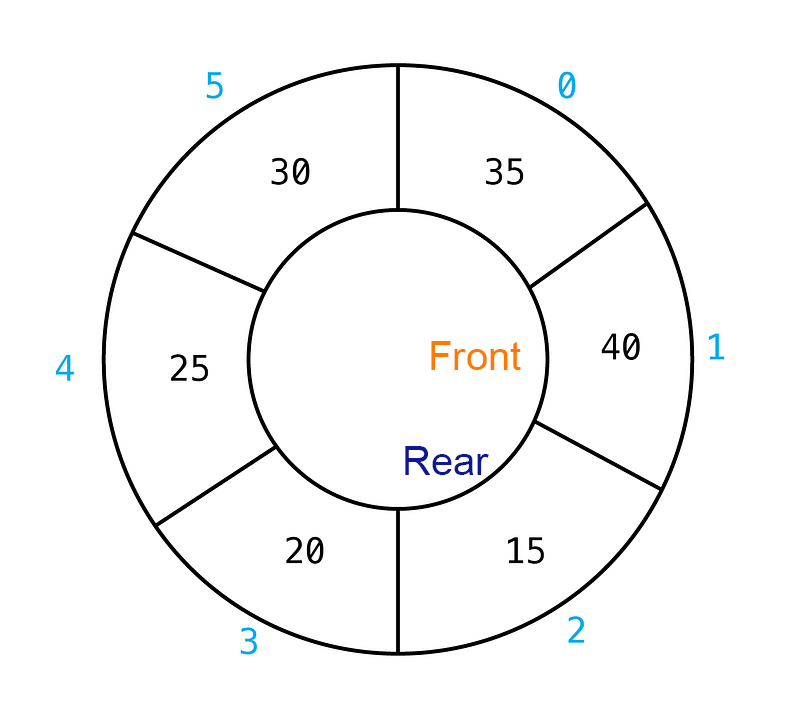
\includegraphics[scale=0.25]{../image/ringbuffer1.png}
              \caption{リングバッファによるキュー}
              \label{img:ringqueue}
            \end{center}
          \end{figure}
        % kasih gambar ring buffer


    
    \subsection{実行環境}
    本実験で使用される実行環境:
    \begin{screen}
        \begin{itemize}
            \item プロセッサ:AMD Ryzen 5 5600X
            \item メモリー:16.0 GB
            \item OS:Windows 11 Pro
            \item コンパイラ:gcc
        \end{itemize}    
    \end{screen}

\section{深さ優先検索と幅優先検索を用いて検索}
    \subsection{深さ優先検索}
    深さ優先探索は,木やグラフのデータ構造を探索するアルゴリズムである.このアルゴリズムは,根(始点)から開始し,バックトラックする前に各辺に沿って可能な限り探索する.

    指定した辺に沿ってこれまでに発見されたノードを追跡し,グラフのバックトラックに役立てるために,スタックが必要となる.

        \subsubsection{深さ優先検索のプログラム}
        以下は深さ優先検索のプログラムである.
        \lstinputlisting[language=c]{D:/Kosen/jikkenII/netgraph/dfs_connect.c} 
        
        \subsubsection{深さ優先検索のプログラムの動作}
        訪問したすべての点はスタックにプッシュされ,その点から先に行けない場合はスタックトップがポップされる.
        深さ優先検索のプログラムの主な流れは,以下の通りである:
        \begin{screen}
            \begin{enumerate}
                \item 根をスタックにプッシュする.
                \item スタックトップのデータを現在点になるようにピークする.
                \item 現在の点に隣接している最も低い点に訪問する.
                \item 現在点から行き場所はない場合,スタックからポップする.
                \item 全ての点を訪問されるまで繰り返す.
            \end{enumerate}
        \end{screen}
        
    \subsection{幅優先検索}
    幅優先探索は,木やグラフのデータ構造を探索するアルゴリズムである.このアルゴリズムは,根(始点)から開始し,各点に隣接している点を訪問する.

    キューは,訪問されたがまだ探索されていない点を追跡するために必要である.

        \subsubsection{幅優先検索のプログラム}
        以下は深さ優先検索のプログラムである.
        \lstinputlisting[language=c]{D:/Kosen/jikkenII/netgraph/bfs_connect.c} 
        
        \subsubsection{深さ優先検索のプログラムの動作}
        訪問したすべての点はキューの\textit{rear}にエンキューされ,その点から先に行けない場合はキューの\textit{front}からデキューされる.
        幅優先検索のプログラムの主な流れは,以下の通りである:
        \begin{screen}
            \begin{enumerate}
                \item 根をキューにエンキューする.
                \item キューの\textit{front}のデータを現在点になるようにピークする.
                \item 現在の点に隣接している全ての点を訪問する.
                \item 現在点から行き場所はない場合,キューからデキューする.
                \item 全ての点を訪れるまで繰り返す.
            \end{enumerate}
        \end{screen}
        
    \subsection{深さ優先検索と幅優先検索の結果}
    この問題では,検索対象となるデータが複数用意されている.両プログラムを実行した結果,下表のような結果が得られました.
    \begin{longtable}[c]{|c|l|l|l|}
        \caption{深さ優先検索結果}
        \label{tab:dfsres}\\
        \hline
        \rowcolor[HTML]{C0C0C0} 
        \cellcolor[HTML]{C0C0C0}Data & \multicolumn{1}{c|}{\cellcolor[HTML]{C0C0C0}Height} & \multicolumn{1}{c|}{\cellcolor[HTML]{C0C0C0}Leaf Count} & \multicolumn{1}{c|}{\cellcolor[HTML]{C0C0C0}Max Child} \\ \hline
        \endfirsthead
        %
        \endhead
        %
        search\_100d.dat      & 99         & 1      & 2   \\ \hline
        search\_100s.dat      & 89         & 8      & 2   \\ \hline
        search\_500d.dat      & 498        & 2      & 3   \\ \hline
        search\_500s.dat      & 483        & 13     & 3   \\ \hline
        search\_1000d.dat     & 999        & 1      & 2   \\ \hline
        search\_1000s.dat     & 982        & 14     & 3   \\ \hline
    \end{longtable}
    \begin{longtable}[c]{|c|l|l|l|}
        \caption{幅優先検索結果}
        \label{tab:bfsres}\\
        \hline
        \rowcolor[HTML]{C0C0C0} 
        \cellcolor[HTML]{C0C0C0}Data & \multicolumn{1}{c|}{\cellcolor[HTML]{C0C0C0}Height} & \multicolumn{1}{c|}{\cellcolor[HTML]{C0C0C0}Leaf Count} & \multicolumn{1}{c|}{\cellcolor[HTML]{C0C0C0}Max Child} \\ \hline
        \endfirsthead
        %
        \endhead
        %
        search\_100d.dat      & 2          & 94      & 66   \\ \hline
        search\_100s.dat      & 4         & 70      & 14   \\ \hline
        search\_500d.dat      & 2        & 495      & 345   \\ \hline
        search\_500s.dat      & 3        & 453     & 50   \\ \hline
        search\_1000d.dat     & 2        & 993      & 607   \\ \hline
        search\_1000s.dat     & 2        & 946     & 108   \\ \hline
    \end{longtable}

    \subsection{深さ優先検索と幅優先検索の考察}
    表(\ref{tab:dfsres})と表(\ref{tab:bfsres})を見ればわかるように,どちらのアルゴリズムも木を生成するが,その特性は異なる.すべてをまとめるために,この表の特徴を以下に記す.

    \begin{longtable}[c]{|c|l|l|}
        \caption{幅優先検索と幅優先検索の特性}
        \label{tab:characteristic}\\
        \hline
        \rowcolor[HTML]{C0C0C0} 
        \cellcolor[HTML]{C0C0C0}特性 & \multicolumn{1}{c|}{\cellcolor[HTML]{C0C0C0}深さ優先検索} & \multicolumn{1}{c|}{\cellcolor[HTML]{C0C0C0}幅優先検索} \\ \hline
        \endfirsthead
        %
        \endhead
        %
        高さ        & 高い    & 低い          \\ \hline
        葉の数       & 少ない   & 多い          \\ \hline
        子の数       & 少ない   & 多い          \\ \hline
    \end{longtable}

    結論として,深さ優先検索は木が長くなるが,各点の子数は少なくなる.
    一方,幅優先検索は木が低くなりますが,各点の子数は多くなります.

\vspace{30pt}
    
\section{連結成分数}
連結成分とは,点の各対が辺で結ばれている部分グラフのことである.
この問題では,与えられたデータがどれだけの連結成分を持つかを数えるというものである.
    
    \subsection{連結成分数のプログラム}
    この問題に対して,新しいプログラムはないので,プログラムのある部分だけに焦点を当てるつもりである.

    以下は深さ優先検索のプログラムである.
    \lstinputlisting[language=c]{D:/Kosen/jikkenII/netgraph/dfs_no3.c} 

    以下は幅優先検索のプログラムである.
    \lstinputlisting[language=c]{D:/Kosen/jikkenII/netgraph/bfs_no3.c} 
    
    \subsection{連結成分数のプログラムの動作}
    検索問題でも同じプログラムを利用する.このデータには複数の連結要素があるので,スタックやキューが空になるが,この処理はまだ終わっていない.なので,未訪問の点を追加しなければならない.両アルゴリズムの主な流れは,以下の通りである:
    \begin{screen}
        \begin{enumerate}
            \item データ構造が空になるまでプログラムを実行する
            \item すべての点を訪問したかどうかをチェックする.
            \item そうでない場合は,最下位の未訪問点をデータ構造に追加する.
            \item すべての点を訪問するまで繰り返す
        \end{enumerate}
    \end{screen}
    言い換えれば,連結成分数を数えるには,この処理が何回繰り返されたかを数えればいい.
    
    \subsection{連結成分数のプログラムの実行結果}
    これらのプログラムを実行した結果,以下のような結果が得られた.
    \begin{screen}
        \begin{itemize}
            \item 深さ優先検索 : 6つ連結成分
            \item 幅優先検索 : 6つ連結成分
        \end{itemize}
    \end{screen}
    
    \subsection{連結成分数の結果の考察}
    表からわかるように,どのようなアルゴリズムで連結成分をチェックしても結果は同じである.
    
\section{最大クリーク問題}
クリークとは部分グラフのことで,すべての点が部分グラフの他のどの点とも辺でつながっているのことである.
言い換えれば,最大クリークはより大きなクリークの部分グラフではないクリークである.
% Clique is a subgraph is a graph in which every vertex is connected by an edge to any other vertex in the subgraph.
% a maximal clique is a clique that cannot be extended by including an additional adjacent vertex; in other words a maximal clique is a clique that is not a subset of a larger clique.

    \subsection{最大クリークのプログラム}
    以下は深さ優先検索のプログラムである.
    \lstinputlisting[language=c]{D:/Kosen/jikkenII/netgraph/clique.c} 
        
    \subsection{最大クリークのプログラムの動作}
    この問題のプログラムは,実際にはピボットなしのブロンケルボッシュアルゴリズムの実装です.しかし,このコードを作るために修正した点がいくつかある.このアルゴリズムは集合の共通部分と和集合を利用するので,すべてのデータを実際の数値として格納する代わりに,各データが配列の添え字として扱った.つまり,ある配列の値0の場合,その値のデータは存在しない,1の場合はその値のデータは存在する.

    ブロンケルボッシュアルゴリズムは以下の通りである.
    \begin{shadebox}
        \texttt{algorithm BronKerbosch1(R, P, X) is \\
        \hspace{10pt} if P and X are both empty then \\
        \hspace{30pt} report R as a maximal clique \\
        \hspace{10pt} for each vertex v in P do \\
        \hspace{30pt} BronKerbosch1(R $\bigcup$ {v}, P $\bigcap$ N(v), X $\bigcap$ N(v)) \\
        \hspace{30pt} P := P $\backslash$ {v} \\
        \hspace{30pt} X := X $\bigcup$ {v}
        }
    \end{shadebox}
   
    
    \subsection{最大クリークの結果}
    この問題では,いくつかのデータを用意した.このプログラムをすべてのデータに対して実行結果は次のようにである. % mungkin hitung waktu eksekusinya aja
    \begin{longtable}[c]{|c|r|r|}
        \hline
        \rowcolor[HTML]{C0C0C0} 
        \cellcolor[HTML]{C0C0C0}Data & \multicolumn{1}{c|}{\cellcolor[HTML]{C0C0C0}Number of Maximal Clique} & \multicolumn{1}{c|}{\cellcolor[HTML]{C0C0C0}Execution Time [s]} \\ \hline
        \endfirsthead
        %
        \endhead
        %
        clique\_30.dat   & 182       & 0.009       \\ \hline
        clique\_50.dat   & 966       & 0.026       \\ \hline
        clique\_70.dat   & 4276      & 0.123       \\ \hline
        clique\_100.dat  & 18138     & 1.358       \\ \hline
    \end{longtable}
    
    \subsection{最大クリークの考察}
    点数が多ければ多いほど,最大クリークも多くなり,その数を数えるのに時間がかかる.
    
    そのため,各反復においてピボットを選択することで,このアルゴリズムを改善することができる.ピボットは,アルゴリズムが行う再帰的呼び出しの回数を最小化するために選択され,ピボットを行わないバージョンのアルゴリズムと比較して,実行時間の節約は大きくなる\cite{bib:cazals}. %liat sitasi ini di bron kerbosch algorithm page wiki

\section{発表者の感想}
    Ntar ini mah

    \begin{thebibliography}{99}
        \bibitem{bib:wikigraph}
        https://en.wikipedia.org/wiki/Graph\_theory(参照2023-07-25)
        \bibitem{bib:boyoh}
        柴田望洋,C言語で学ぶアルゴリズムとでーた構造,SB Creative,2017.
        \bibitem{bib:cazals}
        Cazals, F. \& Karande, C., "A note on the problem of reporting maximal cliques", Theoretical Computer Science, 2008
      \end{thebibliography}
    
\end{document}